\chapter{Appendices for Chapter \ref{chap:strain}}
\label{app:strain}

\section{Hyperparameters for self-training performance at fixed $n_l$}
\label{app:strain:sec:expfixednl}
This section provides a detailed list of the chosen hyperparameters foreach dataset. Self-training hyperparameters can be found in Table \ref{app:strain:tab:sthyperparamsfixednl}. The other hyperparameters are listed in Table \ref{app:strain:tab:otherhyperparamsfixednl}.

\begin{table}
    \centering
    \caption{Training hyperparameters used for the experiments of Section \ref{ssec:strain:fixednl}.}
    \begin{tabular}{|c|ccccc|}
        \hline
        Dataset & $n_l$ & iter/epoch & tile size & $W$ & $E$ \\
        \hline
        \acrshort{monuseg} & $2$ & $100$ & $512$ & $10$ & $50$ \\
        \acrshort{segpc} & $30$ & $300$ & $512$ & $10$ & $50$ \\
        \acrshort{glas} & $8$ & $225$ & $384$ & $10$ & $50$ \\
        \hline
    \end{tabular}
    \label{app:strain:tab:sthyperparamsfixednl}
\end{table}

\begin{table}
    \centering
    \caption{Self-training hyperparameters used for the experiments of Section \ref{ssec:strain:fixednl} for \acrshort{monuseg}  and \acrshort{segpc}. The same hyperparameters have been used for \acrshort{glas}except for the combination ``\textit{constant}'' and $C=0.2$.}
    \begin{tabular}{|cccc|ccc|}
        \hline
        \multirow{2}{*}{}{Weight} & \multirow{2}{*}{}{$C$} & \multirow{2}{*}{}{$w_{min}$} & \multirow{2}{*}{}{$\eta$} & \multicolumn{3}{c|}{Datasets} \\
        & & & & M & S & G \\
        \hline
        constant & $0.01$ &  & & \checkmark & \checkmark & \\
        constant & $0.5$ &  & & \checkmark & \checkmark & \checkmark\\
        constant & $1.0$ &  & & \checkmark & \checkmark & \checkmark\\
        constant & $2.0$ &  & & & \checkmark & \\
        entropy &  & $0.1$ & & \checkmark & \checkmark & \checkmark\\
        consistency &  &  & $2$ & \checkmark & \checkmark & \checkmark\\
        merged &  & $0.1$ & $2$ & \checkmark & \checkmark & \checkmark \\
        \hline
    \end{tabular}
    \label{app:strain:tab:otherhyperparamsfixednl}
\end{table}

\section{Additional weighting strategies evaluated for the fixed $n_l$ experiment}
\label{app:strain:sec:additionalfixednl}

This section reports performance for all the weighting schemes actually evaluated (see Figures \ref{app:strain:fig:rho_exp_monuseg}, \ref{app:strain:fig:rho_exp_segpc} and \ref{app:strain:fig:rho_exp_glas}) for the fixed $n_l$ experiment.

\begin{figure}
    \centering
    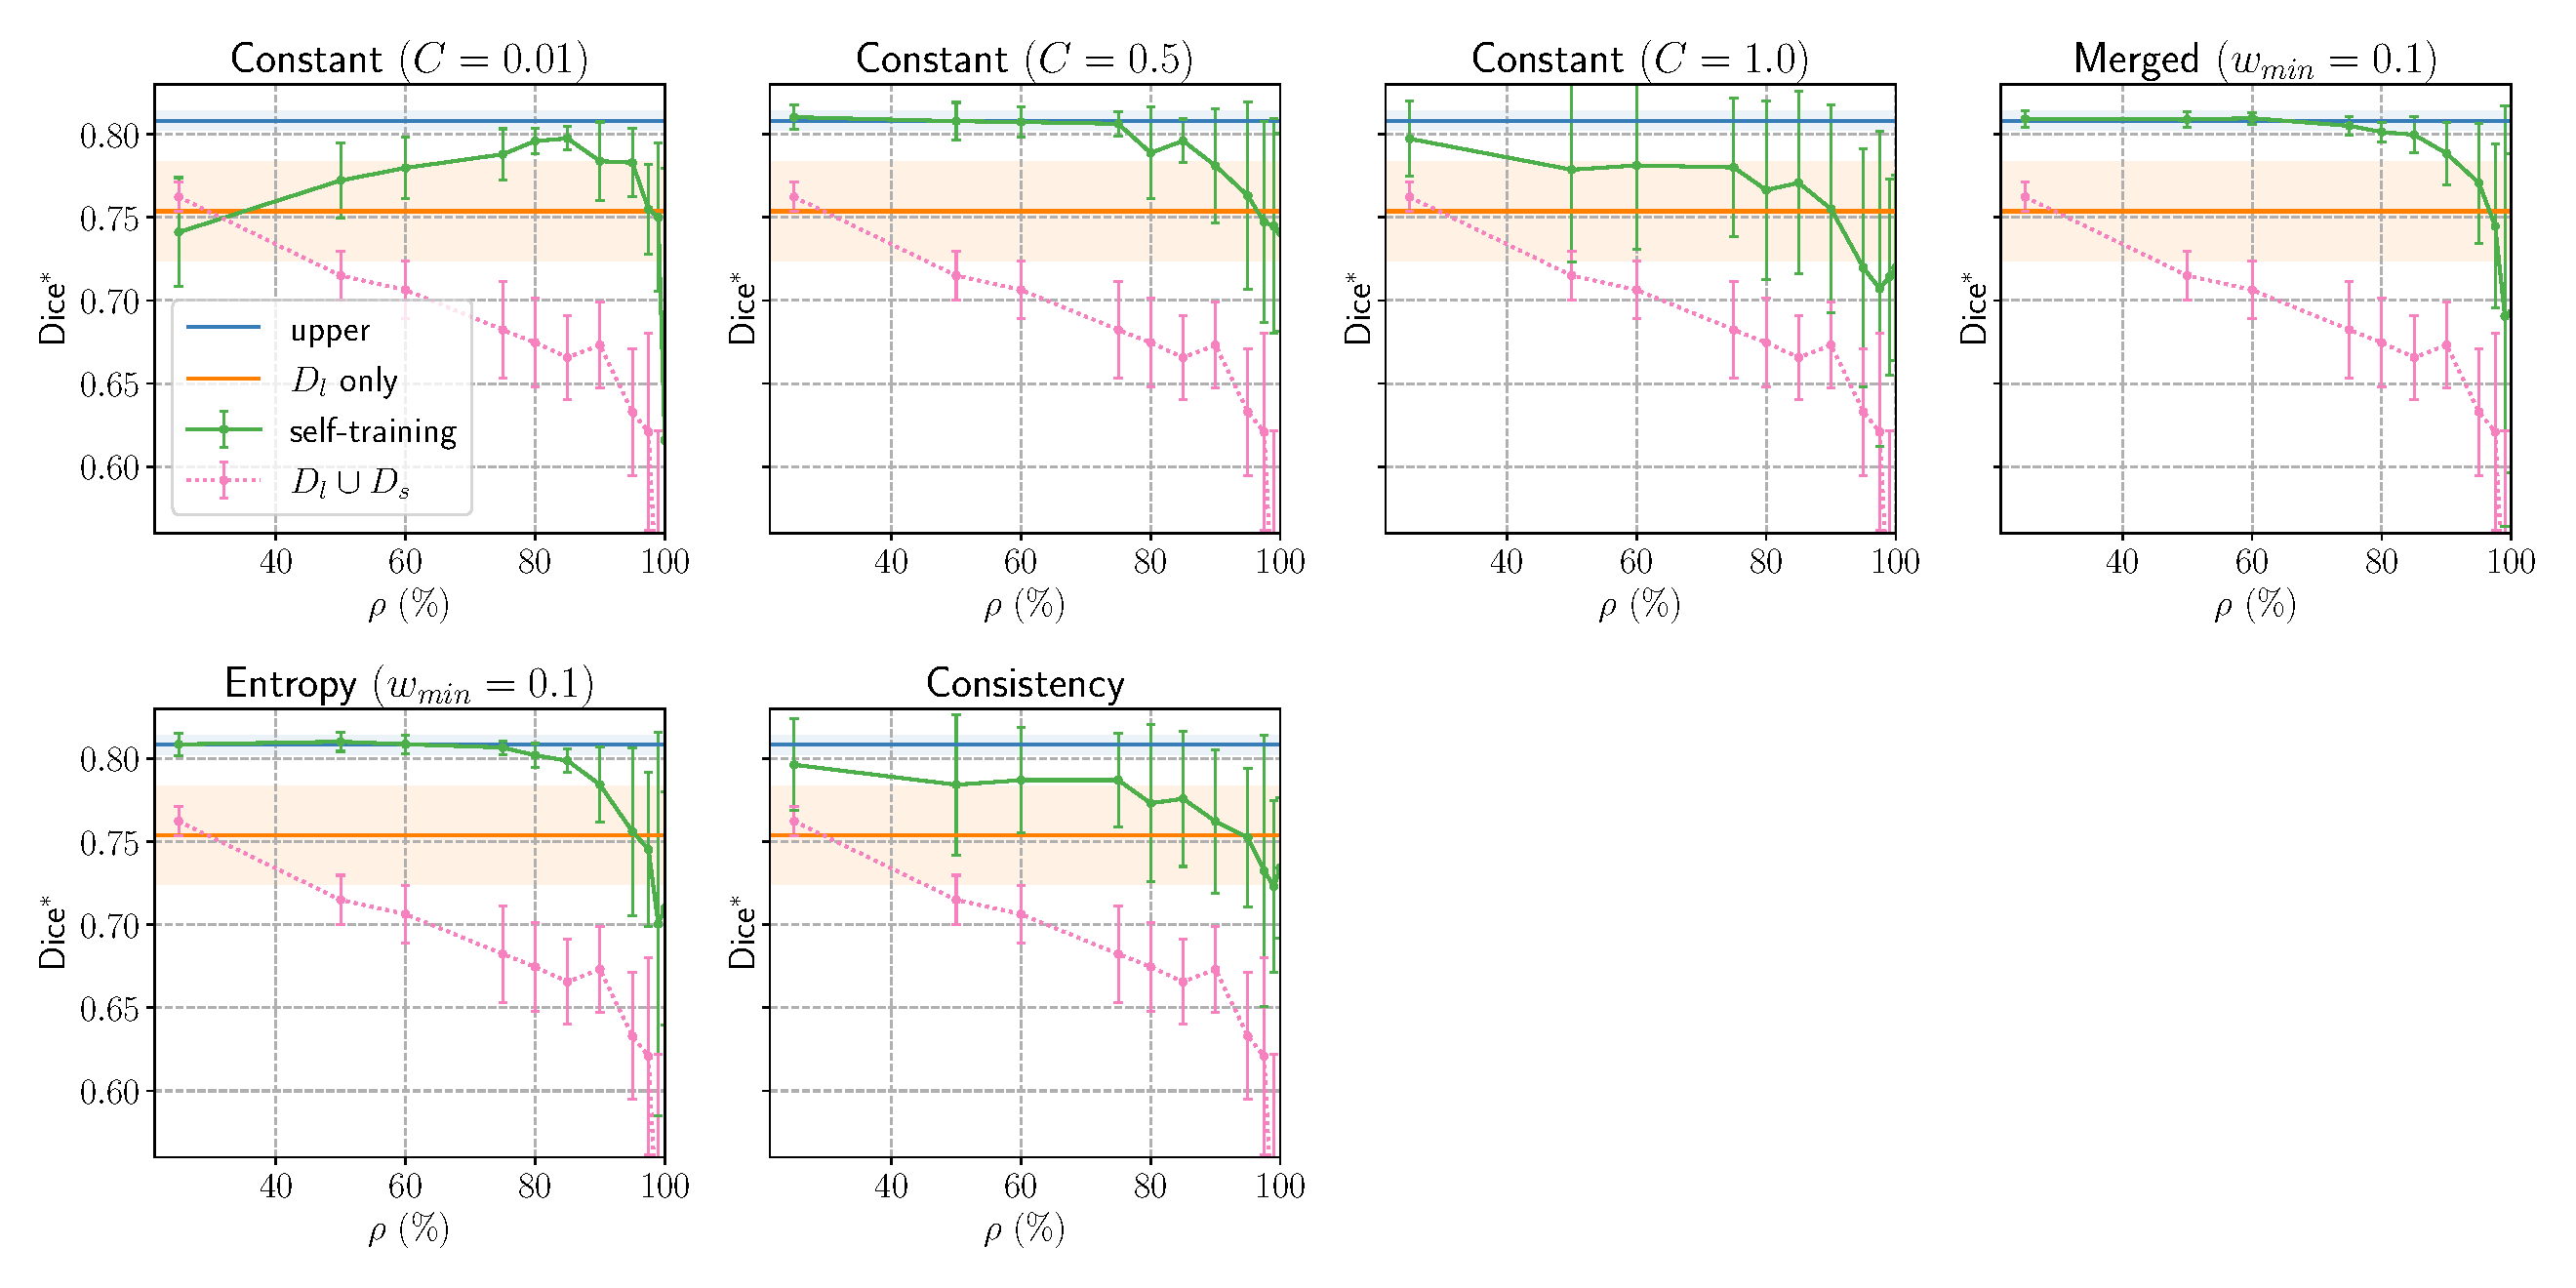
\includegraphics[width=\textwidth]{strain/all_monuseg_test_pxl_self_hard_dice_rho.pdf}
    \caption{\acrshort{monuseg}, see Figure \ref{fig:strain:rho_exp} for explanation.}
      \label{app:strain:fig:rho_exp_monuseg}
\end{figure}

\begin{figure}
    \centering
    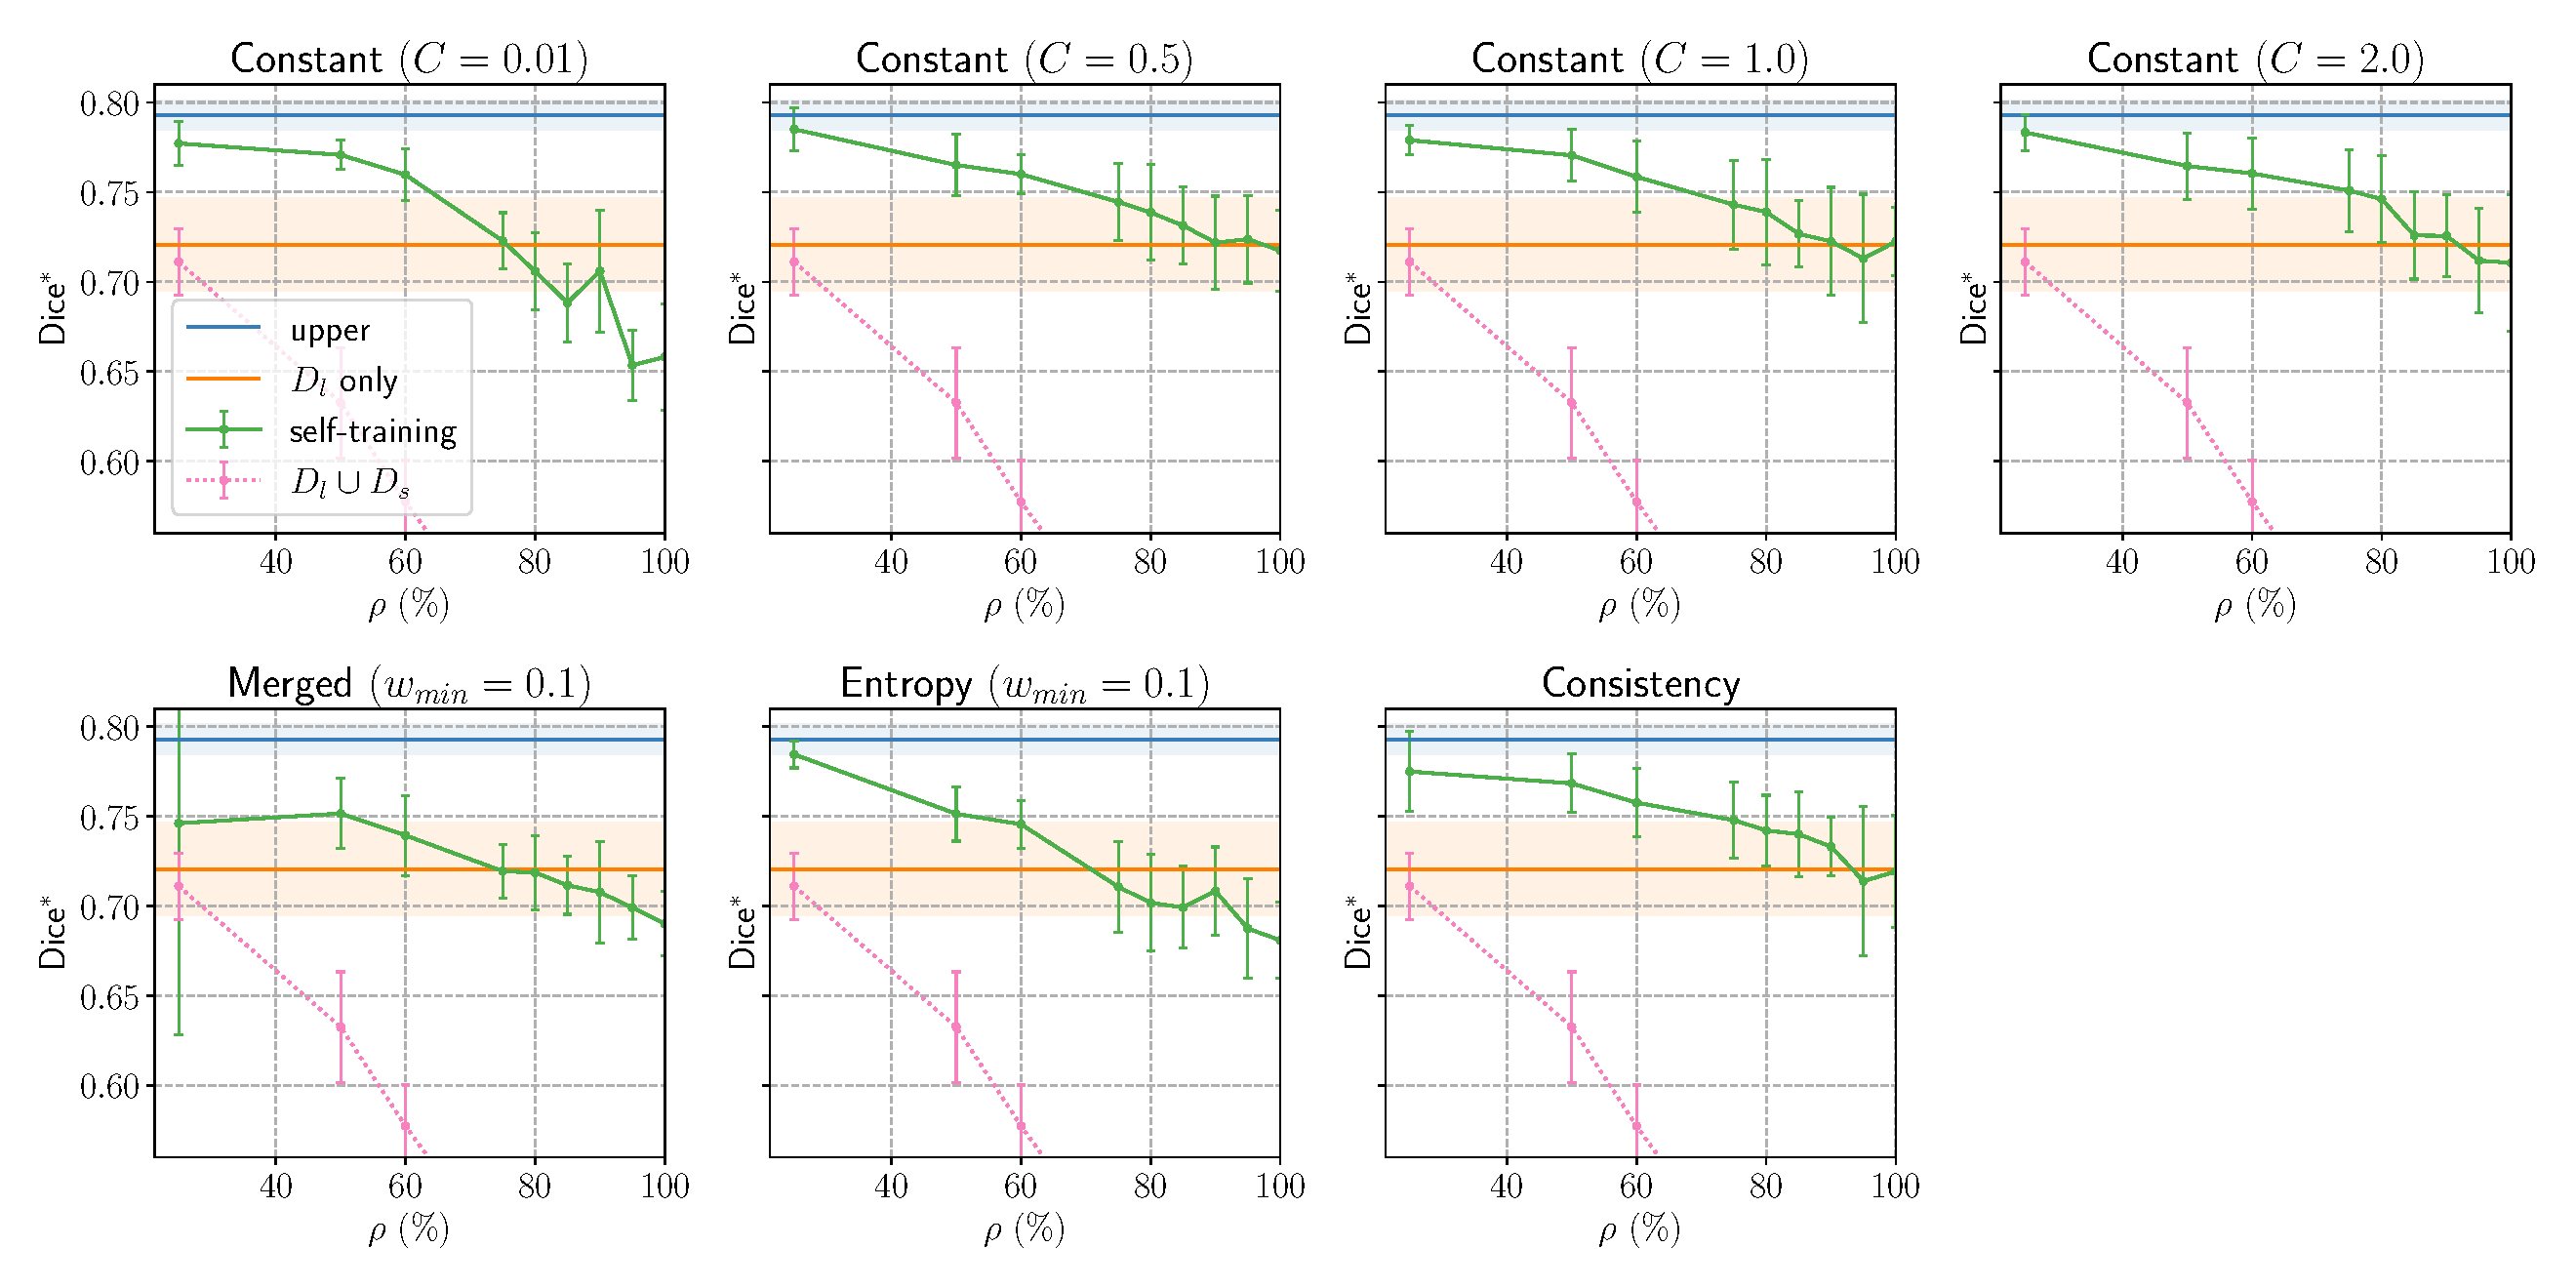
\includegraphics[width=\textwidth]{strain/all_segpc_test_pxl_self_hard_dice_rho.pdf}
    \caption{\acrshort{segpc}, see Figure \ref{fig:strain:rho_exp} for explanation.}
    \label{app:strain:fig:rho_exp_segpc}
\end{figure} 

\begin{figure}
    \centering
    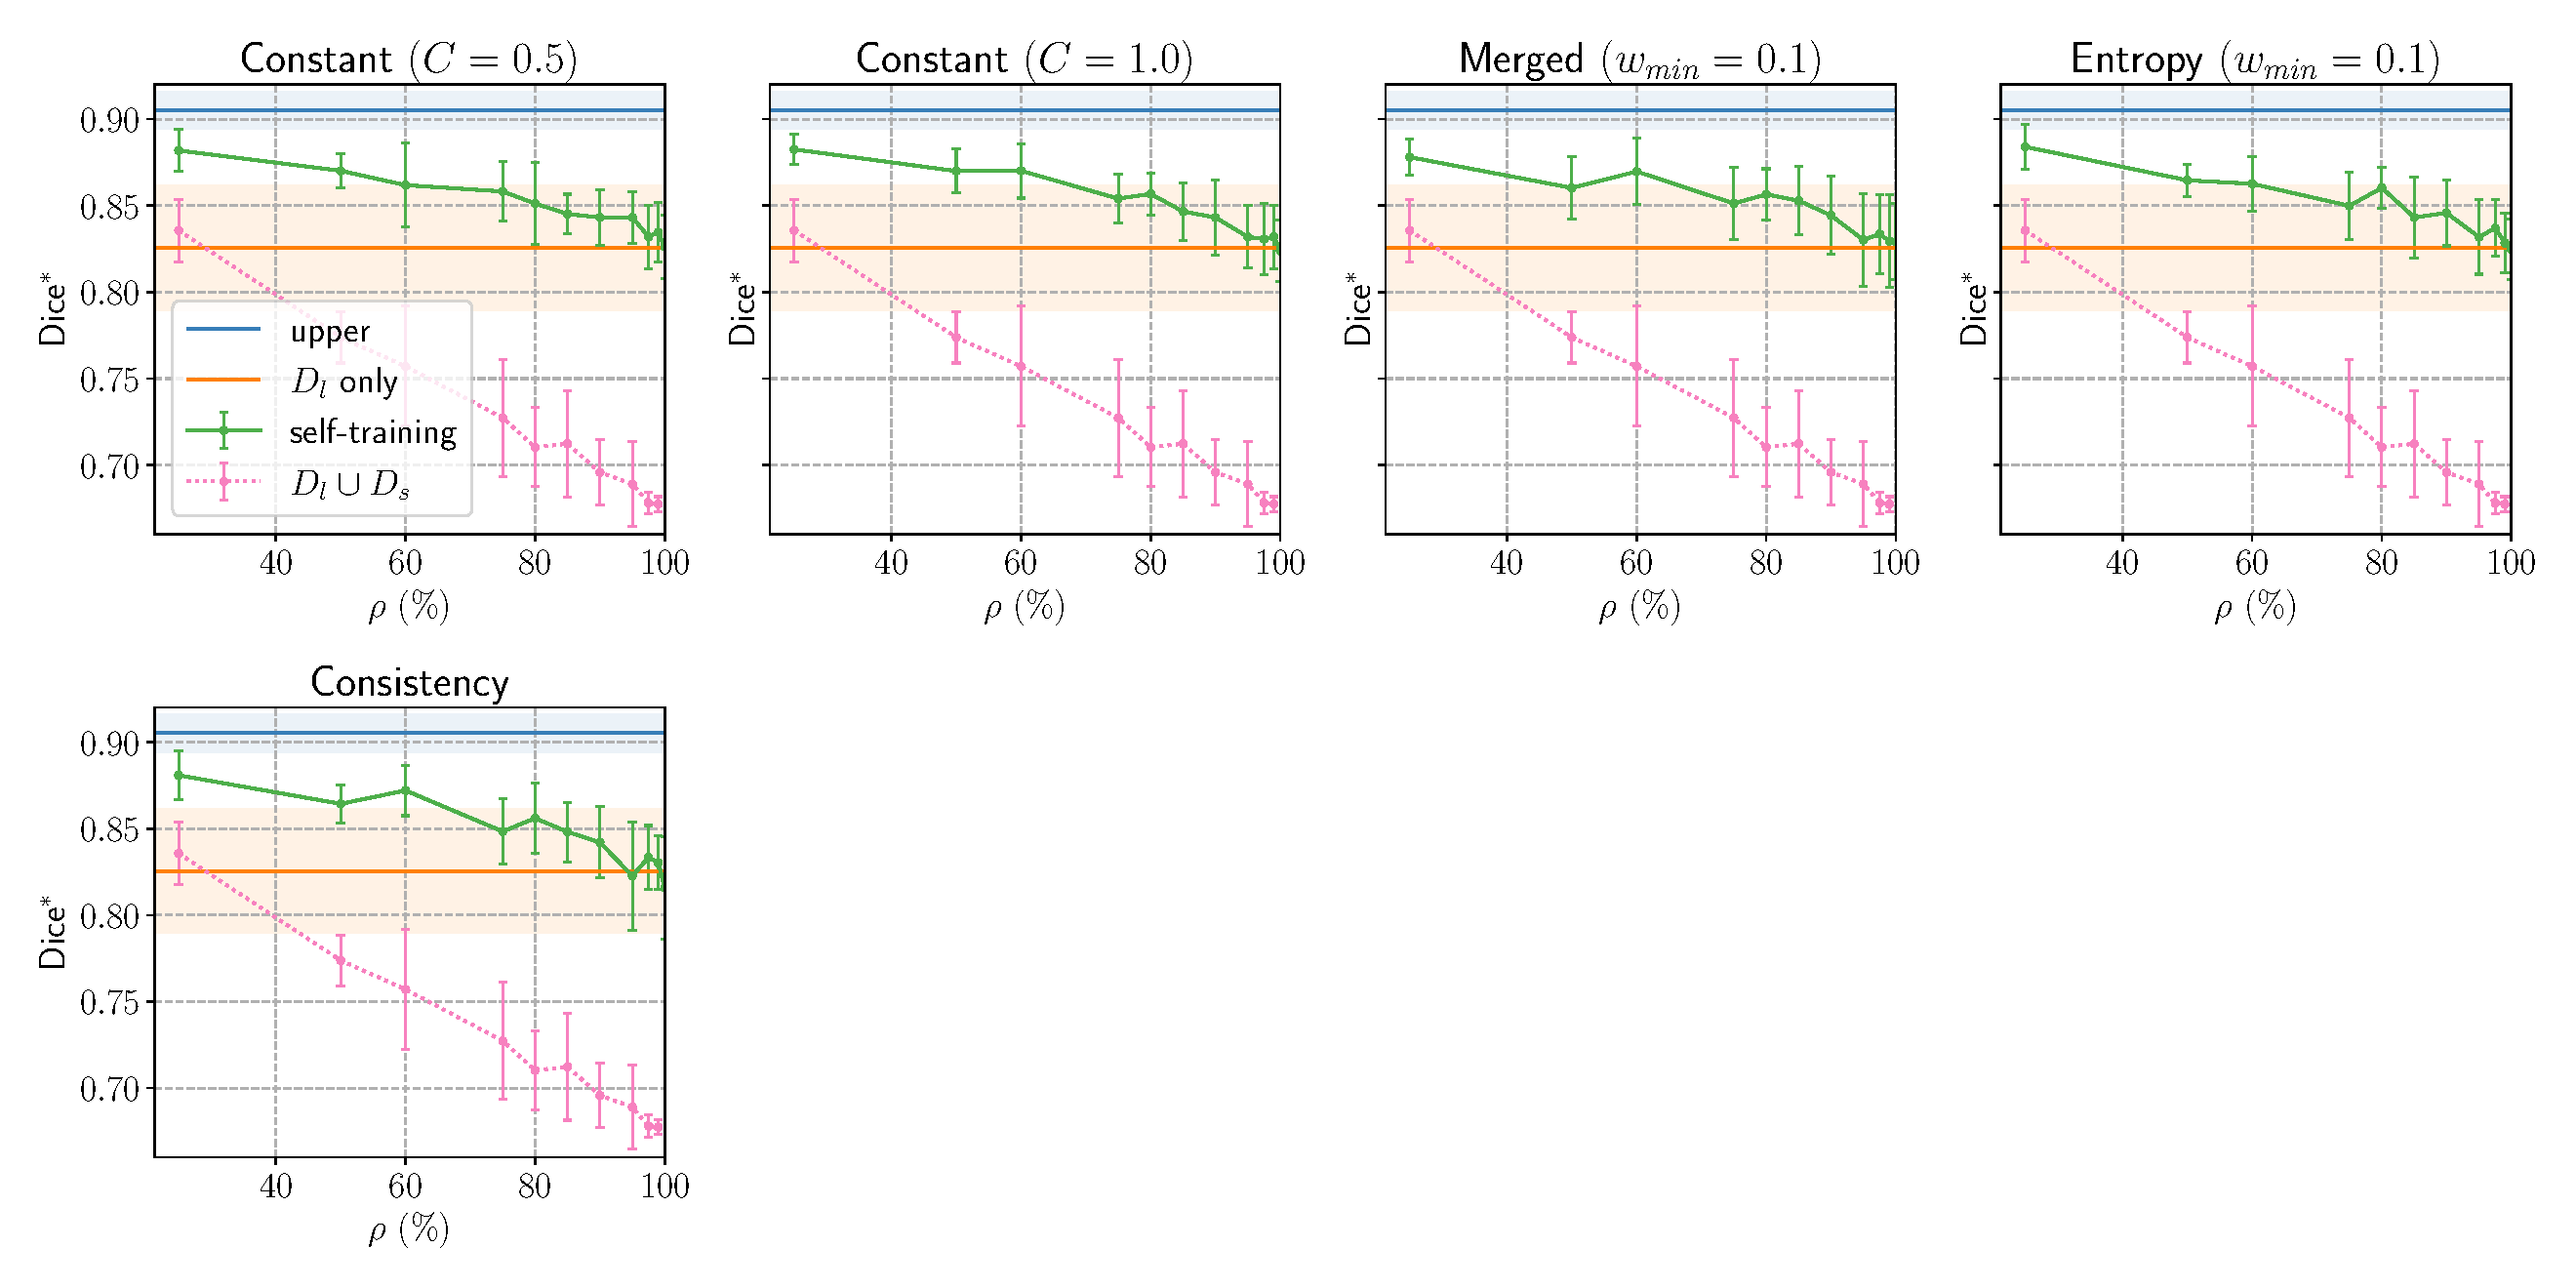
\includegraphics[width=\textwidth]{strain/all_glas_test_pxl_self_hard_dice_rho.pdf}
    \caption{\acrshort{glas}, see Figure \ref{fig:strain:rho_exp} for explanation.}
    \label{app:strain:fig:rho_exp_glas}
\end{figure}
  
\section{About splitting Thyroid \acrshort{fnab} training set into $\mathcal{D}_l$ and $\mathcal{D}_s$}
\label{app:strain:sec:thyroidsplit}

The Thyroid \acrshort{fnab} dataset was labeled by experienced pathologists who followed a detailed ontology to categorize their annotations:

% from the team of Isabelle Salmon from Erasme Hospital in Brussels

\begin{enumerate}
	\item Architectural patterns (see examples in Figure \ref{app:strain:fig:patterns_examples}):
	\begin{itemize}
		\item Normal follicular architectural pattern
		\item Proliferative follicular architectural pattern
		\item Proliferative follicular architectural pattern (minor sign)
	\end{itemize}
	\item Nuclear features (see examples in Figure \ref{app:strain:fig:cells_examples}):
	\begin{itemize}
		\item Papillary cell NOS
		\item Normal follicular cells
		\item Normal follicular cell with pseudo-inclusion (artefact)
		\item Papillary cell with ground glass nuclei
		\item Papillary cell with nuclear grooves
		\item Papillary cell with inclusion
	\end{itemize}
	\item Others:
	\begin{itemize}
		\item Macrophages
		\item Red blood cells
		\item PN (polynuclear)
		\item Colloid
		\item Artefacts
		\item Background
	\end{itemize}
\end{enumerate}

Given how the labeling process was carried out, we hypothesize that crops of architectural patterns are less likely to contain unlabeled cells than crops of nuclear features. Indeed, the former usually consist in large polygons delineating areas containing cell aggregates. Nuclear features, unlike architectural patterns, were usually labeled more sparsely and it is frequent to find annotations of a single cell within an unlabeled cell aggregate. This can be seen in Figures \ref{app:strain:fig:patterns_examples} and \ref{app:strain:fig:cells_examples}. These observations and hypothesis motivate the assignment of architectural patterns to $\mathcal{D}_l$ and nuclear features to $\mathcal{D}_s$.

\begin{figure}
    \centering
    \begin{subfigure}{.48\textwidth}
      \centering
      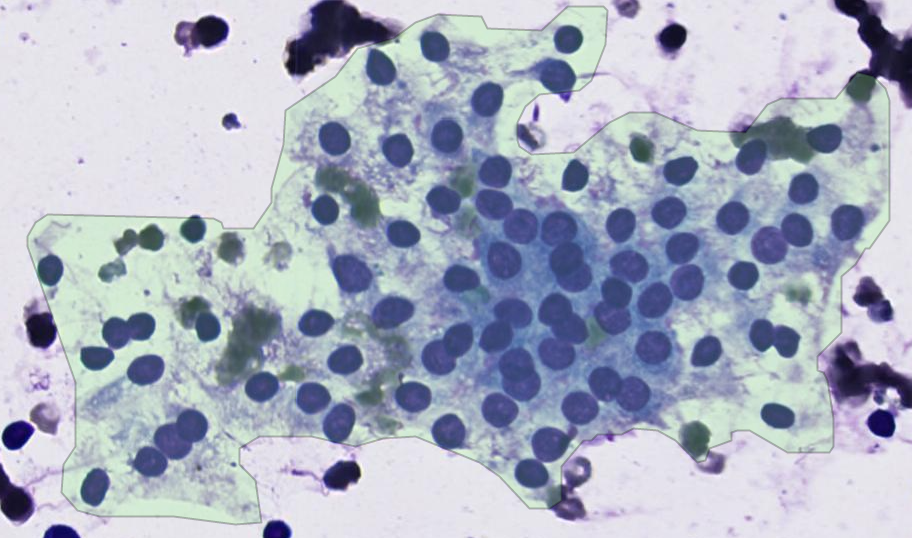
\includegraphics[width=\textwidth]{strain/patterns1.png}
      \caption{}
      \label{app:strain:sfig:pattern1}
    \end{subfigure}
    \begin{subfigure}{.48\textwidth}
      \centering
      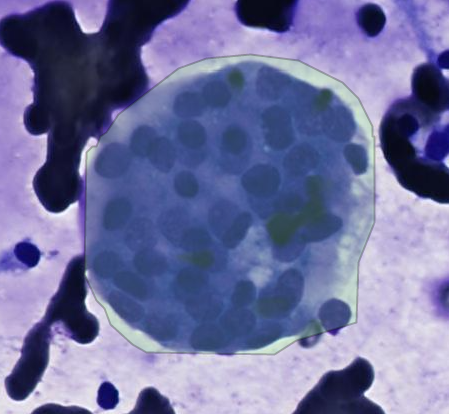
\includegraphics[width=\textwidth]{strain/patterns2.png}
      \caption{}
      \label{app:strain:sfig:pattern2}
    \end{subfigure} \\
    \begin{subfigure}{.48\textwidth}
      \centering
      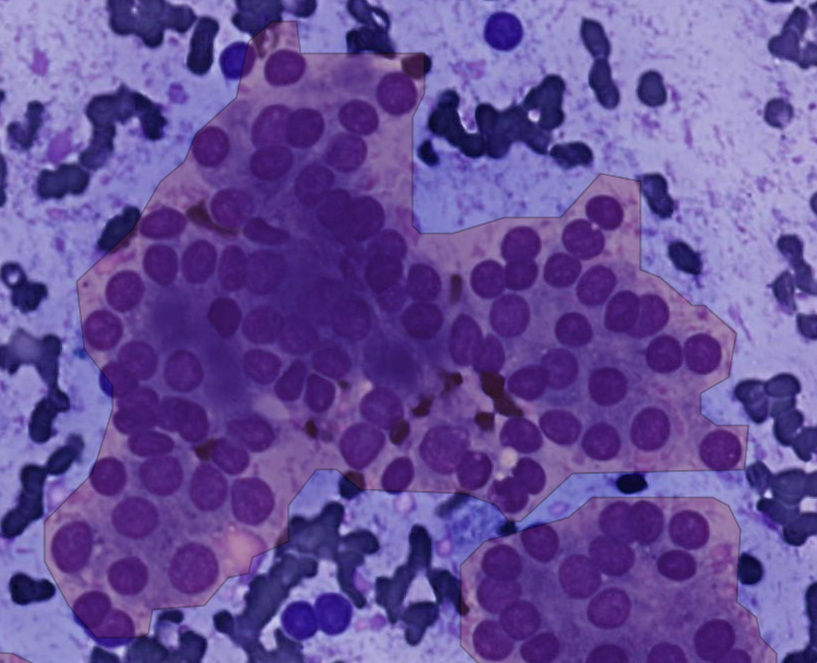
\includegraphics[width=\textwidth]{strain/patterns3.png}
      \caption{}
      \label{app:strain:sfig:pattern3}
    \end{subfigure}
    \begin{subfigure}{.48\textwidth}
      \centering
      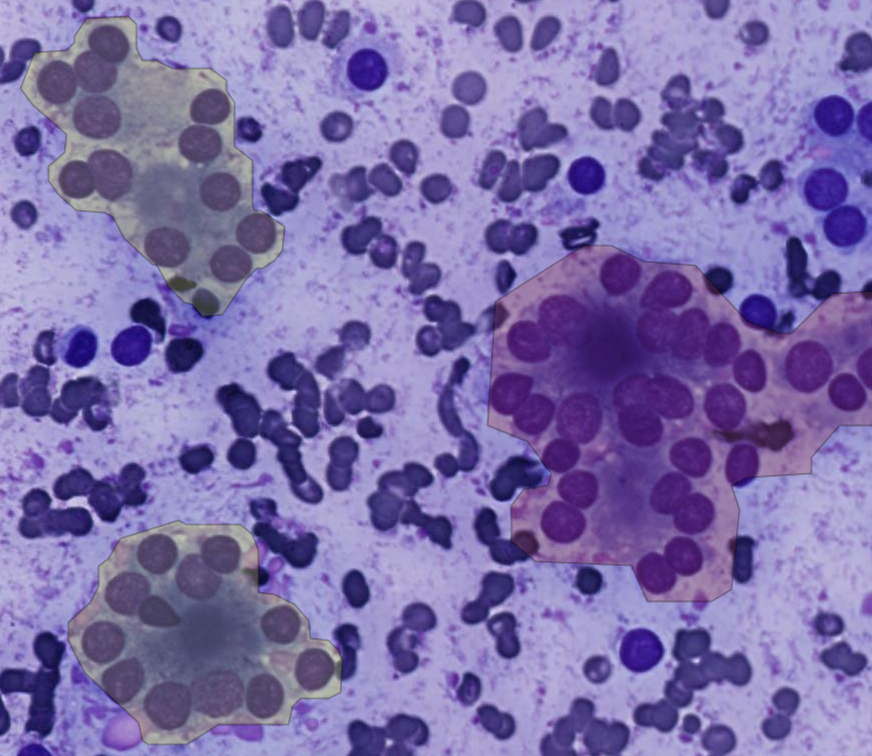
\includegraphics[width=\textwidth]{strain/patterns4.png}
      \caption{}
      \label{app:strain:sfig:pattern4}
    \end{subfigure}
    \caption{Examples of architectural patterns annotations made by pathologists for Thyroid \acrshort{fnab}.}
    \label{app:strain:fig:patterns_examples}
\end{figure}


\begin{figure}
    \centering
    \begin{subfigure}{.235\textwidth}
      \centering
      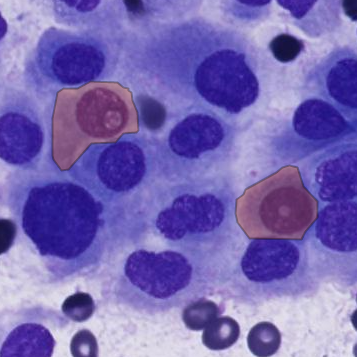
\includegraphics[width=\textwidth]{strain/cells1.png}
      \caption{}
      \label{app:strain:sfig:cell1}
    \end{subfigure}
    \begin{subfigure}{.235\textwidth}
      \centering
      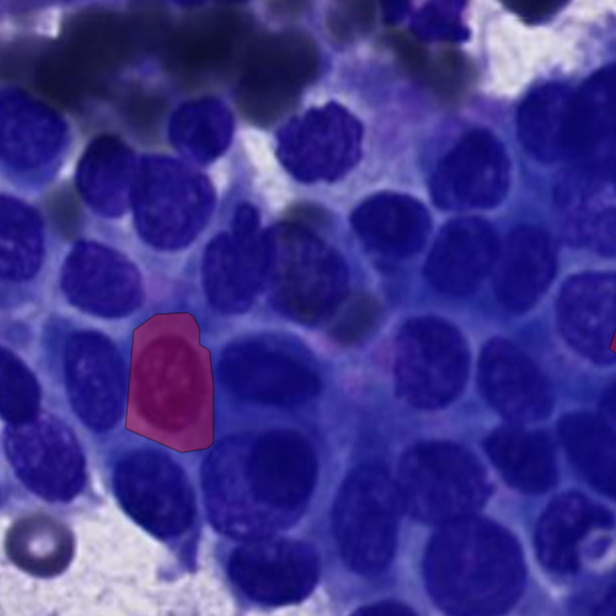
\includegraphics[width=\textwidth]{strain/cells2.png}
      \caption{}
      \label{app:strain:sfig:cell2}
    \end{subfigure}
    \begin{subfigure}{.235\textwidth}
      \centering
      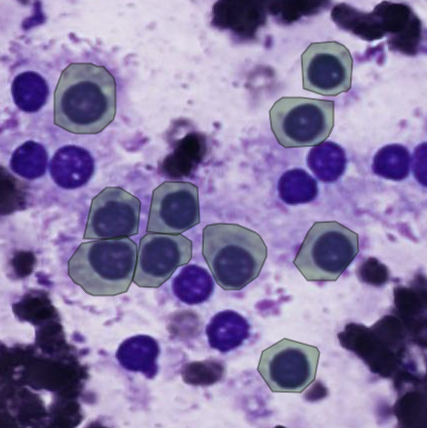
\includegraphics[width=\textwidth]{strain/cells3.png}
      \caption{}
      \label{app:strain:sfig:cell3}
    \end{subfigure}
    \begin{subfigure}{.235\textwidth}
      \centering
      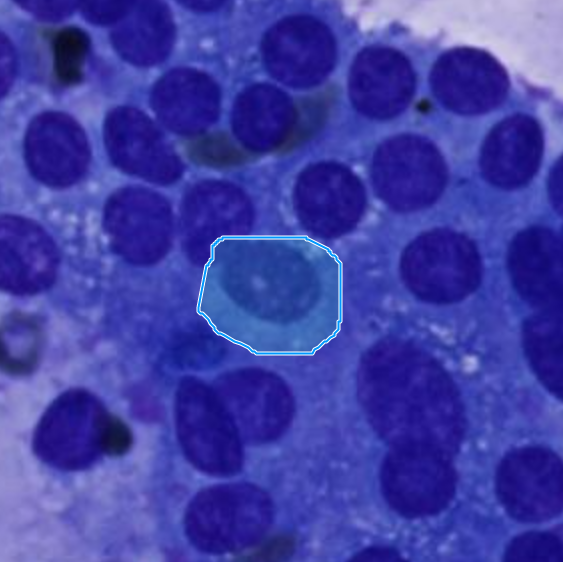
\includegraphics[width=\textwidth]{strain/cells4.png}
      \caption{}
      \label{app:strain:sfig:cell4}
    \end{subfigure}
    \caption{Examples of nuclear features annotations made by pathologists for Thyroid \acrshort{fnab}.}
    \label{app:strain:fig:cells_examples}
\end{figure}

